\documentclass[11pt]{article}

\usepackage{float}
\usepackage[utf8]{inputenc}
\usepackage{hyperref}
\usepackage{graphicx}
\renewcommand{\baselinestretch}{1.1}

\title{Introduction to Word Embeddings (Part 1)}
\author{Aaron Geelon So}
\date{}

\begin{document}
\maketitle

Human language is
\href{https://en.wikipedia.org/wiki/The_Unreasonable_Effectiveness_of_Mathematics_in_the_Natural_Sciences}{unreasonably
effective} at describing how we relate to the world. With a few, short
words, we can convey many ideas and actions with little ambiguity. Well,
\href{http://mentalfloss.com/article/24445/10-amelia-bedelia-isms}{mostly}.

But because we're capable of seeing and describing so much complexity, a
lot of structure is implicitly encoded into our language. It is no easy
task for a computer (or a human, for that matter) to learn \emph{natural
language}, for it entails understanding how we humans observe the world,
if not understanding how \emph{to} observe the world.

For the most part, computers can't understand natural language. Our
programs are still line-by-line instructions telling a computer what to
do. And forget even that, if some blasted semicolon's gone missing.

There's good news though. There's been some important breakthroughs in
\emph{natural language processing} (NLP), the domain where researchers
try to teach computers human language.

Famously, in 2013, Google researchers found a method that enabled a
computer to learn relations between words such as:\footnote{Mikolov
  2013.}
\[\textrm{king} - \textrm{man} + \textrm{woman} \approx \textrm{queen}.\]
This method, called \emph{word embeddings}, has a lot of promise; it
might even be able to reveal hidden structure in the world we see.
Consider one relation it
\href{http://byterot.blogspot.in/2015/06/five-crazy-abstractions-my-deep-learning-word2doc-model-just-did-NLP-gensim.html}{discovered}:
\[\textrm{president} - \textrm{power} \approx \textrm{prime minister}.\]
Admittedly, this might be one of those specious relations.

Joking aside, it's worth studying word embeddings for at least two
reasons. First, there is a lot of applications and avenues for research
made possible by word embeddings. Maybe we can take advantage of their
capabilities if we understand what they are and what they can do. And
second, we can learn from the way researchers approached the problem,
seeing their thought processes as they met and overcame design
challenges.

Let's take a look at the first reason now! We'll go into the theory in
the next \href{2017-07-24-word-embeddings-2.html}{article}.

\subsection*{Uses of Word Embeddings}\label{uses-of-word-embeddings}

There's no obvious useful way to compare two words unless we already
know what they mean. The goal of word-embedding algorithms is therefore
\textbf{to embed words into a space that comes with its own intrinsic
measures of similarity}.

In practice, words are embedded into a real vector space, which comes
with notions of \emph{distance} and \emph{angle}.\footnote{To connect
  back to the previous section, we can think of the dimension \(d\) as
  the number of features we use to encode each word.} We hope that these
notions extend to the embedded words in meaningful ways, quantifying
relations or similarity between different words. And empirically, they
actually do!

For example, the Google algorithm I mentioned above discovered certain
nouns are singular/plural or have gender (Mikolov 2013abc):

\begin{figure}[H]
\centering
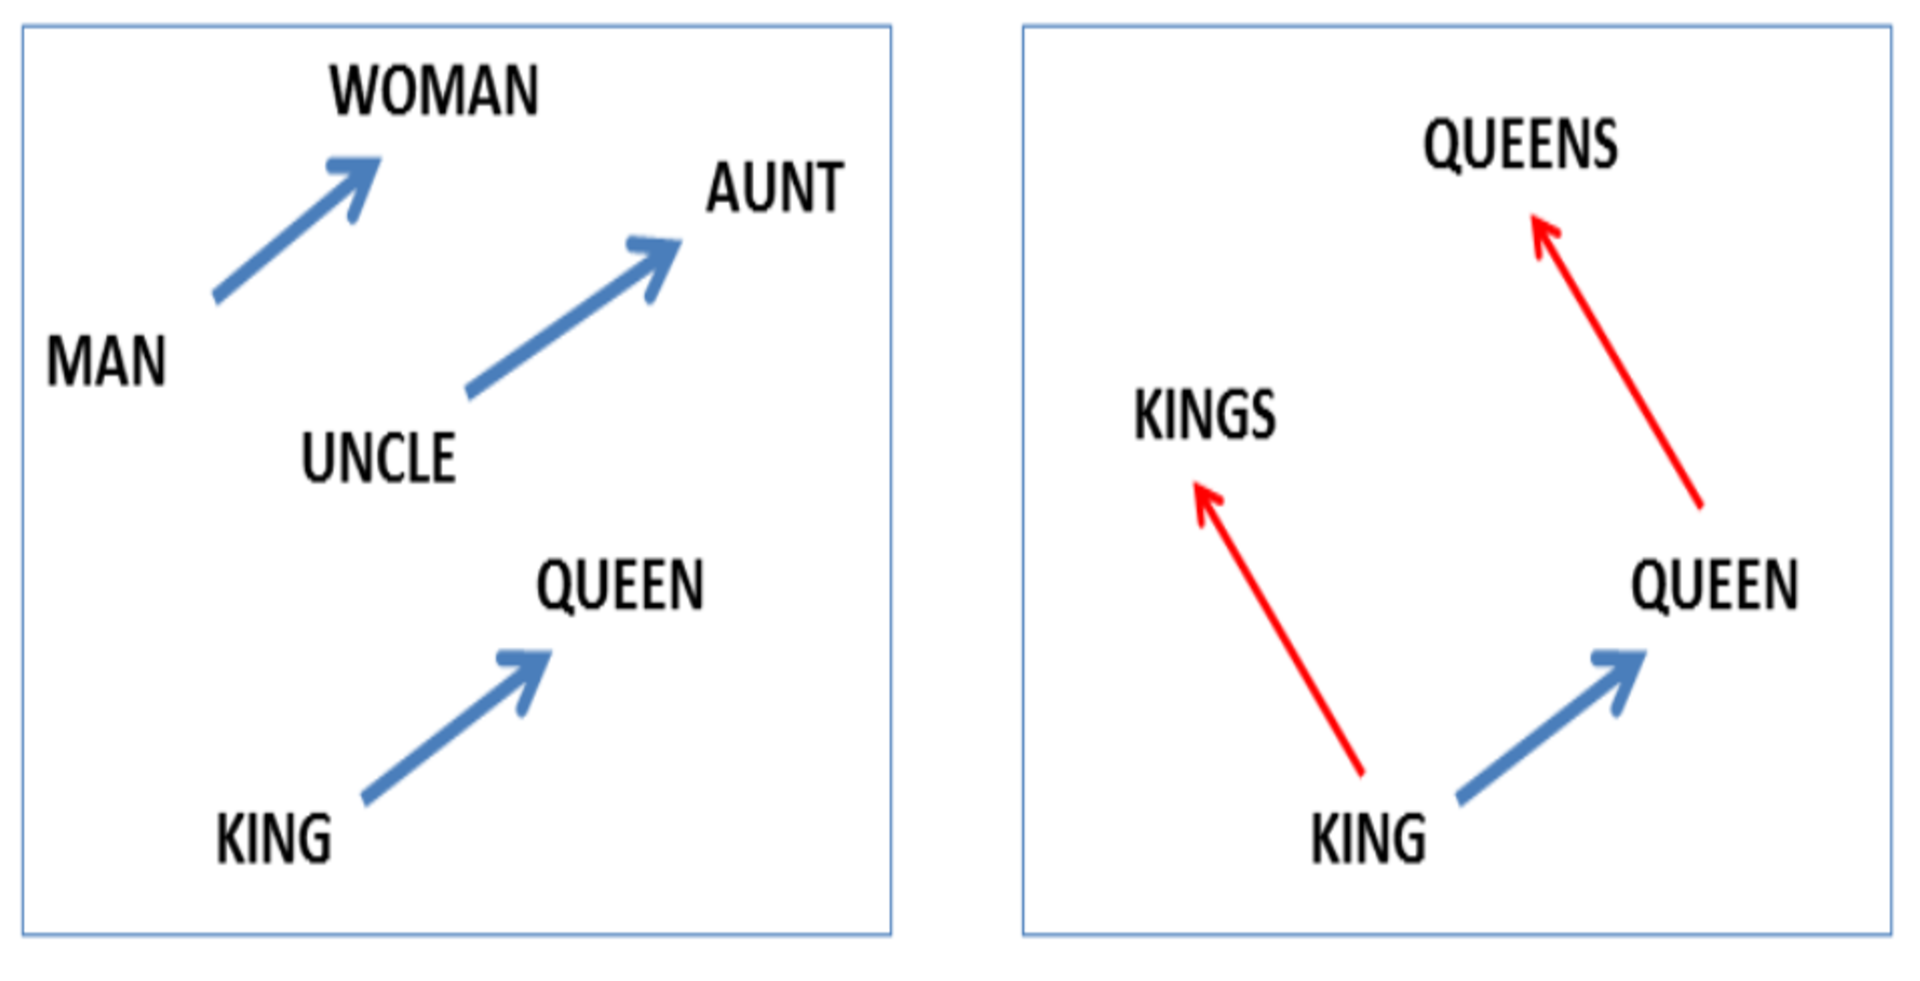
\includegraphics[width=300px]{files/relations.png}
\caption{Projections of word highlighting different relations
captured by the embedding. \emph{Image courtesy of Mikolov 2013a}.}
\end{figure}

They also found a country--capital relationship:

\begin{figure}[H]
\centering
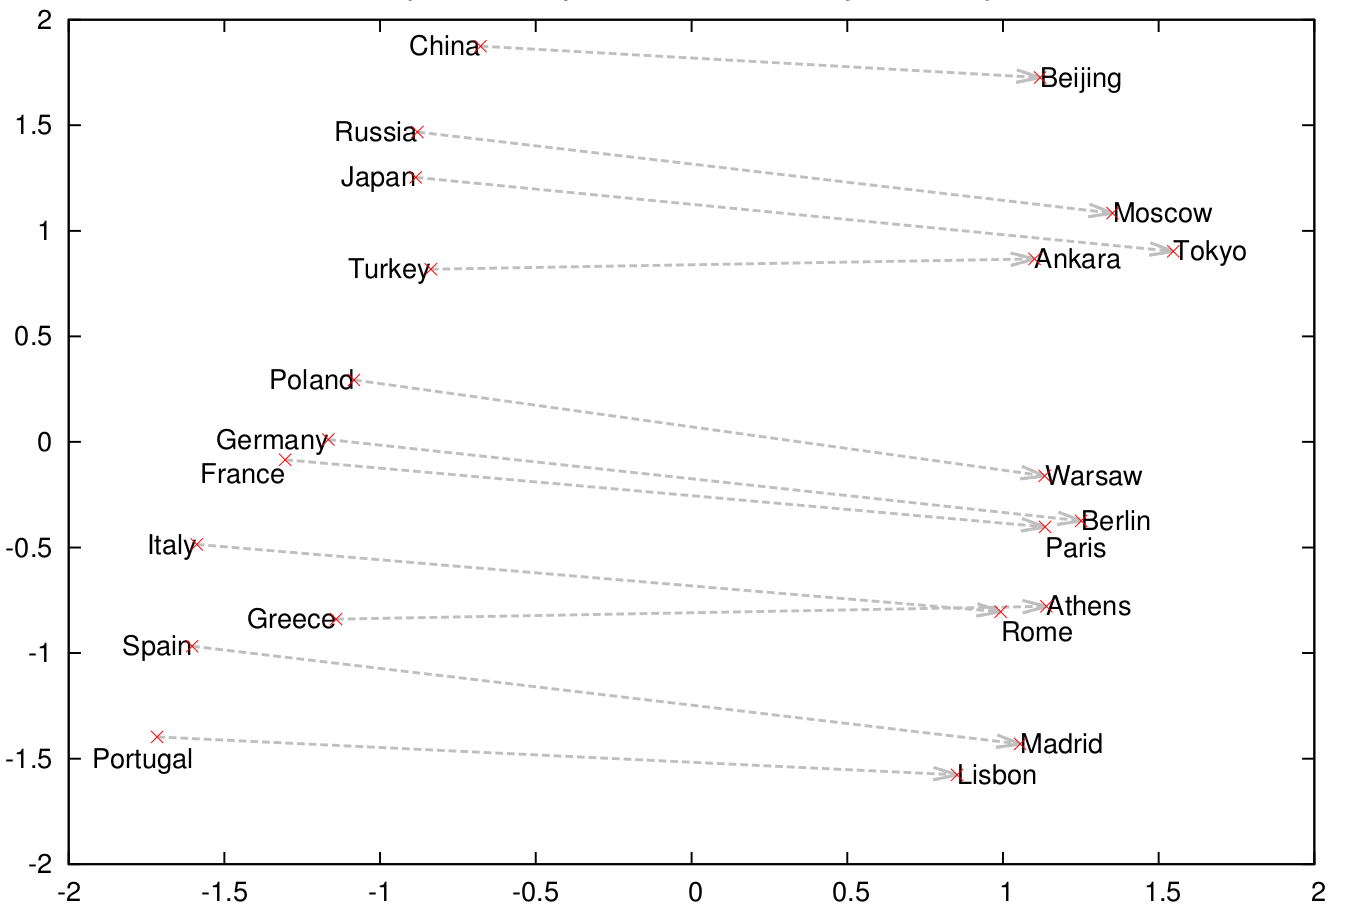
\includegraphics[width=300px]{files/country.png}
\caption{The vectors of few countries and their capitals
projected by PCA. \emph{Image courtesy of Mikolov 2013c}.}
\end{figure}

And as further evidence that meaning comes from the relationships a word
forms, they actually found that the learned structure for one language
often correlated to that of another language, perhaps suggesting the
possibility for
\href{https://en.wikipedia.org/wiki/Machine_translation}{machine
translation} through word embeddings (Mikolov 2013c).

\begin{figure}[H]
\centering
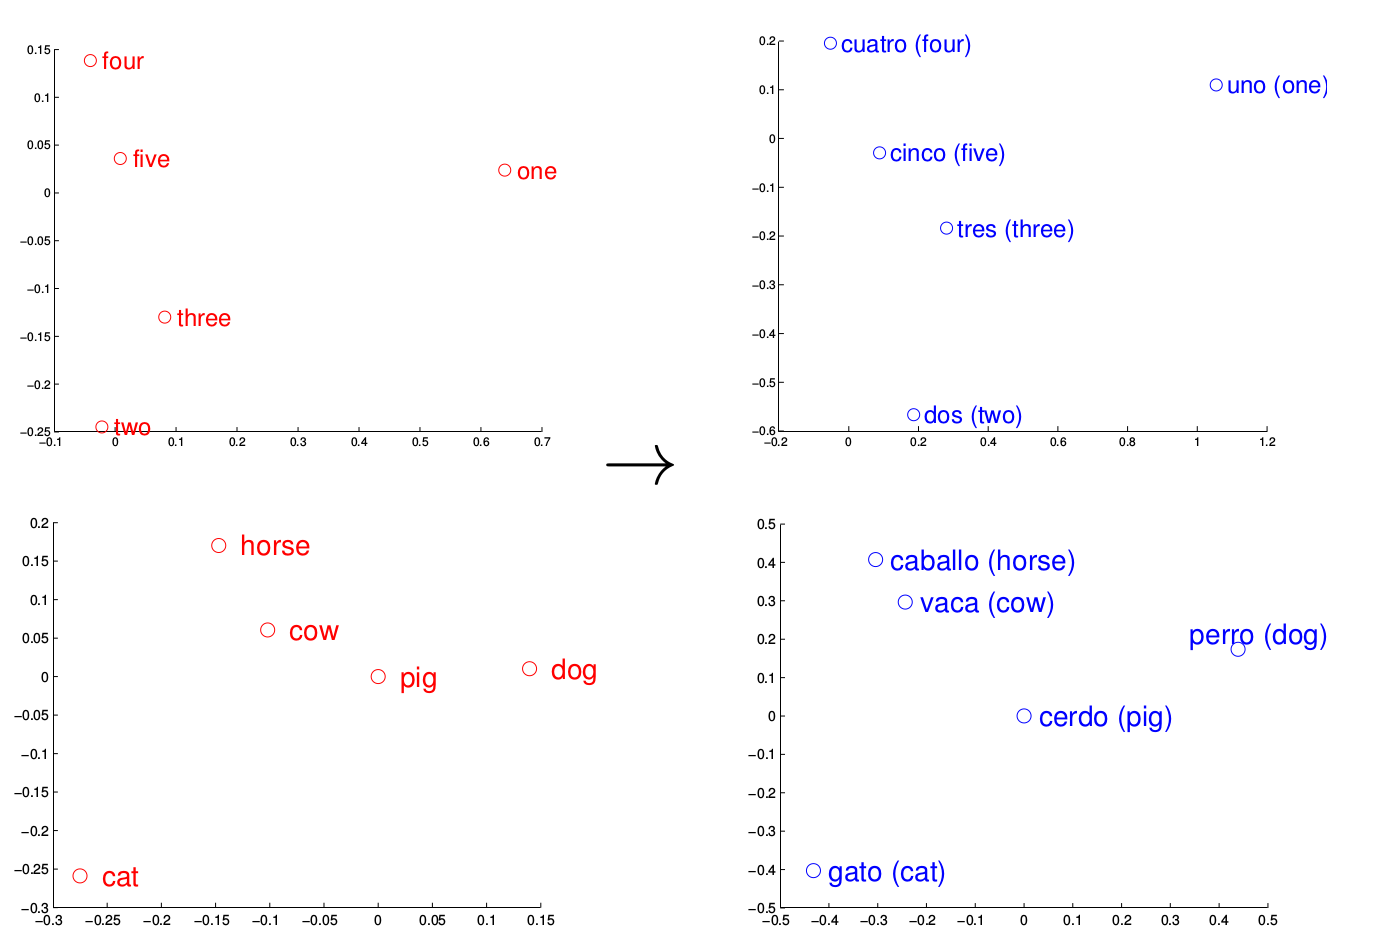
\includegraphics[width=300px]{files/mt.png}
\caption{A comparison of word relations in different
languages. \emph{Image courtesy of Mikolov 2013d}.}
\end{figure}

They released their C code as the
\href{https://code.google.com/p/word2vec}{word2vec} package, and soon
after, others adapted the algorithm for more programming languages.
Notably, for \href{https://radimrehurek.com/gensim/index.html}{gensim}
(Python) and \href{https://deeplearning4j.org/word2vec}{deeplearning4j}
(Java).

Today, many companies and data scientists have found different ways to
incorporate word2vec into their businesses and research.
\href{https://www.slideshare.net/eshvk/spotifys-music-recommendations-lambda-architecture}{Spotify}
uses it to help provide music recommendation.
\href{http://multithreaded.stitchfix.com/blog/2015/03/11/word-is-worth-a-thousand-vectors/}{Stitch
Fix} uses it to recommend clothing. Google is thought to use word2vec in
\href{http://searchengineland.com/faq-all-about-the-new-google-rankbrain-algorithm-234440}{RankBrain}
as part of their search algorithm.

Other researchers are using word2vec for sentiment analysis, which
attempts to identify the emotions words convey. For example, one
\href{https://arxiv.org/pdf/1606.02820.pdf}{Stanford research group}
looked at how the same words in different Reddit communities take on
different connotations.

\begin{figure}[H]
\centering
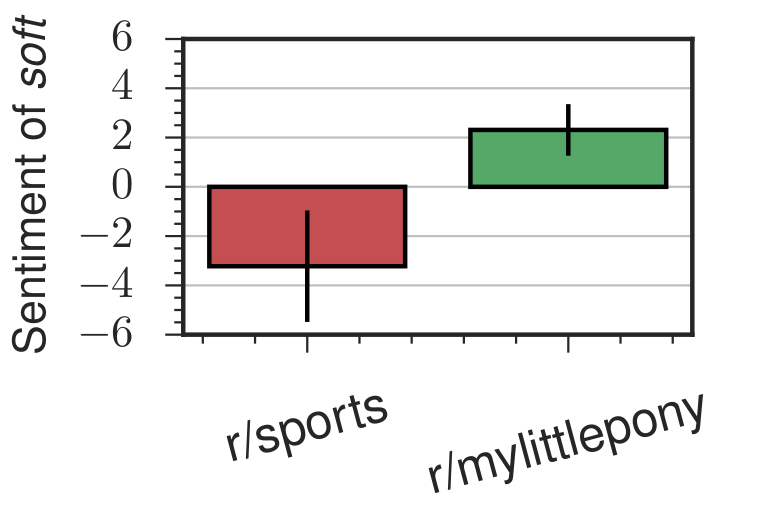
\includegraphics[width=300px]{files/reddit.png}
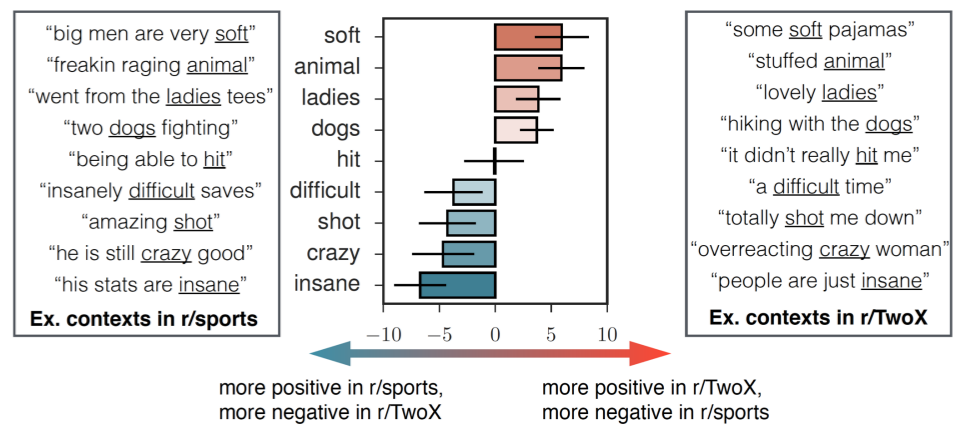
\includegraphics[width=300px]{files/reddit-spectrum.png}
\caption{The same word in different communities can take on
different connotations. \emph{Image courtesy of Hamilton 2016}.}
\end{figure}

They can even apply the same method over time, following how the word
\emph{terrific}, which meant \emph{horrific} for the majority of the
20th century, has come to mean \emph{great} today.

\begin{figure}[H]
\centering
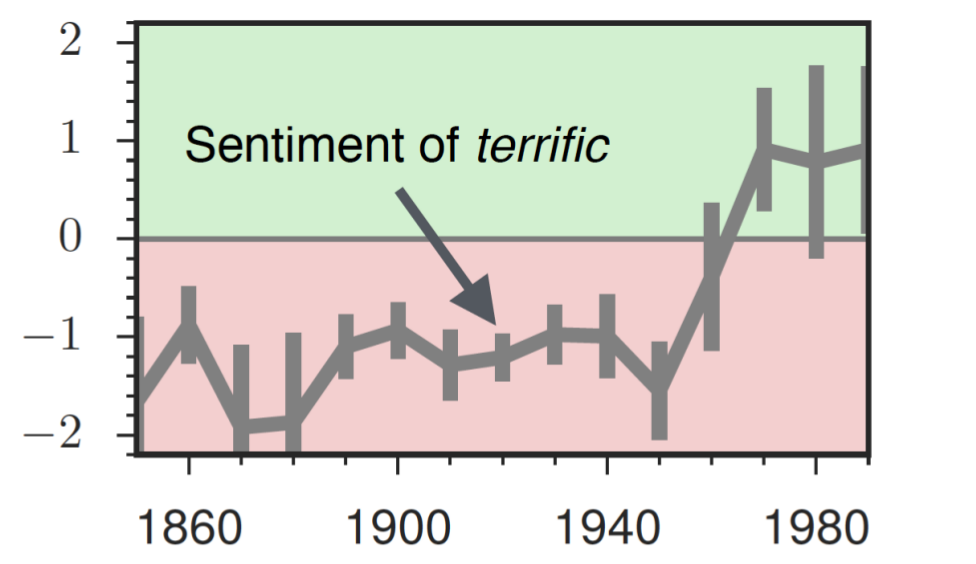
\includegraphics[width=300px]{files/terrific.png}
\caption{The evolution of the word \emph{terrific} over time.
\emph{Image courtesy of Hamilton 2016}.}
\end{figure}

As a light-hearted example, one
\href{http://www.pelleg.org/shared/hp/download/fun-facts-wsdm.pdf}{research
group} used word2vec to help them determine whether a fact is surprising
or not, so that they could automatically generate trivia facts.

The successes of word2vec have also helped spur on other forms of word
embedding---\href{https://arxiv.org/pdf/1506.02761.pdf}{WordRank},
Stanford's \href{https://nlp.stanford.edu/projects/glove/}{GloVe}, and
Facebook's \href{https://research.fb.com/projects/fasttext/}{fastText},
to name a few major ones. But not only do other algorithms seek to
improve on word2vec, they also look at texts through different
\emph{units}: characters, subwords, words, phrases, sentences,
documents, and even perhaps thought.\footnote{A ``thought vector'' is a
  new concept to represent an idea, perhaps more general than a word.
  Here is a blog post on thought vectors on
  \href{https://deeplearning4j.org/thoughtvectors}{deeplearning4j}, and
  here's an research article on
  \href{https://arxiv.org/pdf/1506.06726.pdf}{skip-thought vectors}.
  Here's a neat result from the latter article: out of a
  500,000-sentences corpus, their algorithm could find semantically- and
  syntactically-near sentences. For example, ``im sure youll have a
  glamorous evening, she said, giving an exaggerated wink'' and ``im
  really glad you came to the party tonight, he said, turning to her''.}
As a result, they allows us to think about not just word similarity, but
also sentence similarity and document similarity---like this paper did
(Kusner 2015):

\begin{figure}[H]
\centering
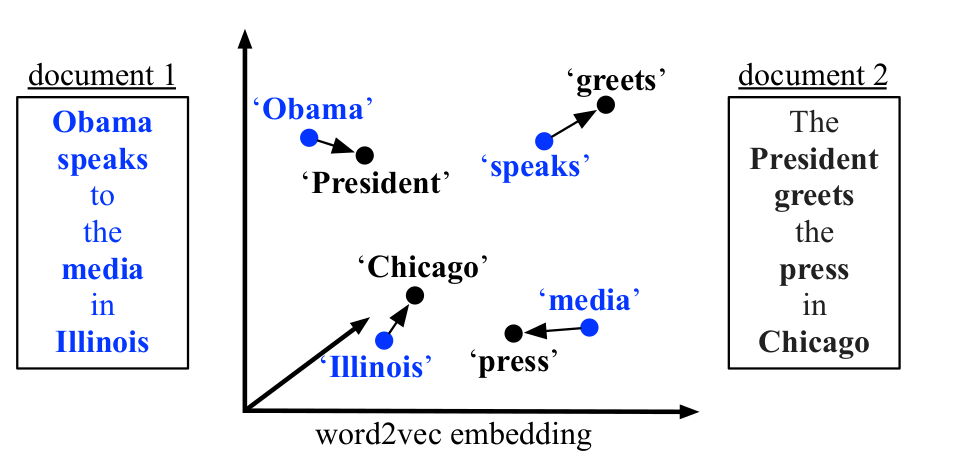
\includegraphics[width=300px]{files/wmd.png}
\caption{The calculation that determines how similar two
sentences are. \emph{Image courtesy of Kusner 2015}.}
\end{figure}

Word embeddings \textbf{transform human language meaningfully into a
form conducive to numerical analysis}. In doing so, they allow computers
to explore the wealth of knowledge encoded implicitly into our own ways
of speaking. Although the lexical data we can now access may give way to
remarkable insight, it is unremarkable that there should be so many
applications. In fact, we've barely scratched the surface.

There's great potential, though, for any individual programmer or
scholar to use these tools and contribute new knowledge. Many areas of
research and industry that could benefit from NLP have yet to be
explored. Word embeddings and neural language models are powerful
techniques. But perhaps the most powerful aspect of machine learning is
its collaborative culture. Many, if not most, of the state-of-the-art
methods are open-source, along with their accompanying
research.\footnote{In fact, not a single one the references I used is
  behind a paywall.}

So, it's there, if we want to take advantage. Now, the main obstacle is
just ourselves. And\ldots{}maybe an expensive GPU.\footnote{Although,
  you could consider cloud services like
  \href{https://aws.amazon.com/}{Amazon Web Services}!}


\end{document}
